\documentclass{beamer}
\usepackage{graphicx}
\usepackage{caption}
\usepackage{subcaption}
\usepackage{color}
\usepackage{listings}
\usepackage{verbatim}
\captionsetup{compatibility=false}
%\usepackage[italian]{babel}  

%% Se per qualsiasi motivo non riuscissi a compilare col tema Unipd,
%% basta commentare la riga qui sotto e si passa automaticamente al
%% tema beamer di default.
\usetheme{Unipd}

\lstdefinestyle{customc}{
  belowcaptionskip=1\baselineskip,
  breaklines=true,
  %frame=L,
  xleftmargin=\parindent,
  language=C,
  showstringspaces=false,
  basicstyle=\fontsize{7}{7}\selectfont\ttfamily,%\footnotesize\ttfamily,
  keywordstyle=\bfseries\color{green!40!black},
  commentstyle=\itshape\color{gray},
  identifierstyle=\color{blue!40!black},
  %stringstyle=\color{orange},
}
\lstset{escapechar=@,style=customc}

\title{Accelerazione GPU nella simulazione/controllo/identificazione di sistemi fisici}
%\subtitle{da inserire}
\author{Diego Casella, Fabio Marcuzzi, Marco Virgulin}
\date{\today}


\begin{document}

\maketitle

\begin{frame}{Contenuti} %Outline
\tableofcontents
\end{frame}

%% Introduzione
\section{Introduzione}
\begin{frame}{Introduzione}

Vogliamo capire come possiamo utilizzare le GPU per accelerare la simulazione/controllo/identificazione di sistemi fisici, e se possibile anche
la co-simulazione.

I problemi sono tutti quelli trattabili da CfL\footnote{ \href{http://www.simnumerica.com/content/what-cfl}{CfL link}} (\dots), pi\'u la co-simulazione di un sistema di controllo.

\end{frame}

\section{Parallelismo massivo}
\begin{frame}{Parallelismo massivo}
- Quanti processori (es. nella nostra scheda abbiamo 7 multiprocessors, ognuno dei quali ha 48 cores) e come si tengono impegnati: 
\begin{itemize}
\item blocks: sono completamente paralleli 
\item threads: possono 
	\begin{itemize}
	\item comunicare (shared memory per i threads di uno stesso blocco; i dati devono transitare per la memoria globale)
	\item sincronizzarsi (tutti i threads devono raggiungere la barriera); 
	\item esempi utili: un thread elabora uno stencil
	\item c'\'e un numero massimo di threads per blocco, da cui il numero di blocchi, detto N dimensione del problema diventa ( \#define BLOCKS (N + (THREADS – 1)) / THREADS )
	\end{itemize}
\end{itemize}

$\rightarrow$ ogni core può eseguire in parallelo un \textit{warp} di threads ! (spesso 32 threads)
\end{frame}


\begin{frame}{Parallelismo massivo}
- il collo di bottiglia della memoria: tutti questi processori devono essere alimentati di operandi ...
\begin{itemize}
\item device (GPU):
	\begin{itemize}
	\item locale
	\item shared
	\item globale (la CPU pu\'o spedire dati solo qui)
	\end{itemize}
\item host (CPU):
	\begin{itemize}
	\item cache I e II livello
	\item principale (RAM)
	\item secondaria (disco)
	\end{itemize}
\end{itemize}

\end{frame}


\begin{frame}[fragile]{Parallelismo massivo}
Esempio 1: PDE

Saltando la generazione di meshes, vediamo la distribuzione della discretizzazione del dominio (mesh) e dei dati del problema:
\begin{lstlisting}
data = zeros((NT,9),dtype = 'float32') # coordinate dei vertici degli elementi in formato  [x11,x12,x13,y11,y12,y13,...]
data[:,0:3] = self.mesh.get_nx()[self.mesh.get_triangles()]
data[:,3:6] = self.mesh.get_ny()[self.mesh.get_triangles()]
data = data.flatten()
...
gal_p1_A(cuda.InOut(data),cuda.Out(idxs),cuda.In(ijk),...,block = (256, 1, 1), grid=(int(np.ceil(NT/256)), 1))
\end{lstlisting}
dove 
\begin{lstlisting}
code = open('gFEM.cu', 'r').read()
mod = SourceModule(code)
gal_p1_A = mod.get_function("compute_A")
\end{lstlisting}
e corrisponde alla chiamata (del modulo CUDA su GPU):
\begin{lstlisting}
compute_A<<<grid, block>>>(float* data, int* idxs, int* ijk, ...)
\end{lstlisting}

\end{frame}


\begin{frame}[fragile]{Parallelismo massivo}
Esempio 1: PDE

- la creazione del modello discreto:
\begin{itemize}
\item la memorizzazione della matrice sparsa;
	\begin{lstlisting}
	scipy.sparse.coo_matrix
	\end{lstlisting}
\item la costruzione delle matrici locali;
	\begin{lstlisting}
	gal_p1_A(cuda.InOut(data),cuda.Out(idxs),cuda.In(ijk),NN,NT,sigma,mu,cuda.In(b),tDt,NN,NT,block = (256, 1, 1), grid=(np.ceil(NT/256), 1))
	\end{lstlisting}
	calcola i contributi dei termini PDE su ogni triangolo della mesh (ad ogni thread viene associato un triangolo).
\item l'assemblaggio;\\
	\begingroup
		\color{blue!40!black}
		\fontsize{9pt}{9pt}
		\verb#thrust::reduce_by_key#
	\endgroup
	\hspace{.1cm}(Thrust library)\\
	per sommare i contributi sui nodi con lo stesso indice (che \'e la chiave).
\end{itemize}


\end{frame}


\begin{frame}[fragile]{Parallelismo massivo}
Esempio 1: PDE

Soluzione del problema discreto con:\\
\begingroup
	\color{blue!40!black}
	\fontsize{9pt}{9pt}
	\verb#cusp::krylov::gmres#
\endgroup
\hspace{.1cm}(Cusp library)\\
Generalized Minimum Residual (GMRES) method.

La libreria viene caricata da \verb@ctypes@ (e contiene al suo interno i moduli CUDA):
\begin{lstlisting}
cusp_so = ctypes.CDLL(FOLDER +'pycusp' + '.so')
cusp_gmres = cusp_so.gmres
...
cusp_gmres(c_ptr(rows_d.ptr),c_ptr(cols_d.ptr),c_ptr(vals_d.ptr),A_coo.shape[0],A_coo.shape[1],A_coo.nnz,c_ptr(b_d.ptr),c_ptr(x_d.ptr),500,ctypes.c_float(1e-6))
\end{lstlisting}

\end{frame}


\begin{frame}[fragile]{Parallelismo massivo}
Esempio 2: Problemi Inversi

\begin{lstlisting}
while (<condizione di terminazione>) {
  ...
  /* Data generation */
  dim3 threadsPerBlockBuild(2, N_delta, N_parameters);
  BuildXtemp<<<1, threadsPerBlockBuild>>>(X_temp, X_temp2, deltatemp, deltatemp2, u, param, param_min, param_max, delta_ini, delta_max);
  ...
  /* Psi generation */
  dim3 threadsPerBlockPsi(N_delta, N_parameters);
  BuildPsi<<<1, threadsPerBlockPsi>>>(Psi, vdiff, X_temp, X_temp2, deltatemp, deltatemp2);
  ...
  /* Gauss-Newton approximation */
  dim3 threadsPerBlockGN(N_updates);
  GN<<<1, threadsPerBlockGN>>>(app_delta, err, u, Psi, vdiff, param, param_min, param_max);
  ...
}
\end{lstlisting}

\end{frame}


\begin{frame}{Parallelismo massivo}
Esempio 3: Linear Algebra
\end{frame}


\begin{frame}{Parallelismo massivo}
Esempio 4: co-simulazioni multiple

- ``multiple (CPU) threads can share a device''.

\end{frame}



\section{Programmazione}
\begin{frame}{Programmazione}
- CUDA: è un'estensione del C per il parallelismo e la gestione del device

\end{frame}


\begin{frame}{Programmazione}
- PyCUDA

\end{frame}


\begin{frame}{Programmazione}
- Thrust

\end{frame}



\section{Tools di sviluppo}
\begin{frame}{Linguaggi ed ambienti di sviluppo}
- nvcc

\end{frame}


\begin{frame}{Linguaggi ed ambienti di sviluppo}
- Marco, puoi scrivere qualcosa sul profiler ?

\end{frame}



\section{Esempi}
\begin{frame}{Esempi}

\begin{figure}
\centering
\begin{subfigure}{.5\textwidth}
  \centering
  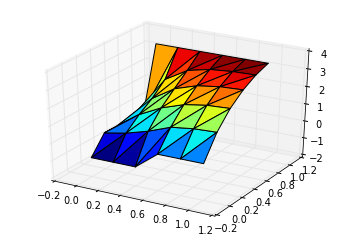
\includegraphics[scale=0.5]{calore.png}
  \caption{Soluzione FEM}
\end{subfigure}%
%\caption{Soluzione FEM}
\end{figure}

- esempi PDE tesi Barasti

\end{frame}


\begin{frame}{Esempi}

- applicazione alla finanza

\end{frame}


\begin{frame}{Esempi}

- tesi Marco su fMRI ?

\end{frame}


\begin{frame}{Esempi}

\end{frame}

\section{Q\&A}
\begin{frame}{Q\&A}
\end{frame}

\end{document}
